\documentclass[sigplan,anonymous,review,nonacm]{acmart}

\renewcommand\footnotetextcopyrightpermission[1]{}
\settopmatter{printfolios=true}
\settopmatter{printacmref=false}
\setcopyright{none}

\usepackage{booktabs}
\usepackage{array}
\usepackage{enumitem}
\usepackage{amsmath}
\usepackage{graphicx}
\usepackage{algorithm}
\usepackage{algpseudocode}
\usepackage{tikz}
\usetikzlibrary{arrows.meta,calc,fit,positioning}

\acmConference[EuroSys '27]{Twenty-Second European Conference on Computer Systems}{April 19--23, 2027}{Rabat, Morocco}
\acmYear{2027}
\acmISBN{}
\acmDOI{}

% The public technical-report title is intentionally distinct from the private
% double-blind submission title. A submission staging directory may provide an
% untracked anonymous-submission-title.tex that renews \papertitle.
\newcommand{\systemname}{Semantic MapReduce}
\newcommand{\papertitle}{\systemname: An Auditable Operator Contract for LLM-Backed Reduction}
\IfFileExists{anonymous-submission-title.tex}{\input{anonymous-submission-title.tex}}{}
\title{\papertitle}

\author{Anonymous Authors}
\affiliation{%
  \institution{Anonymous Institution}
  \country{}
}

\begin{document}
\pagestyle{plain}

\begin{abstract}
Data engines define precise contracts for scans, joins, windows, and aggregation, but an LLM placed above those operators can still change analysis state through unaudited text. The missing contract specifies which records become evidence, which evidence may be fused, which model decisions are admissible, and what state remains after rejection. We present \emph{\systemname{}}, an operator algebra and runtime contract for reducing partitioned observations into evidence-linked hypotheses. Its data-facing operators produce normalized evidence and candidate groups; \textsf{SemanticReduce} produces a valid baseline; a model may implement only a bounded \textsf{Edit} in \{\textsc{Keep}, \textsc{Merge}, \textsc{Split}, \textsc{Abstain}\}; and system-owned \textsf{Validate} and \textsf{ReportTrace} bind evidence identifiers, enforce invariants, preserve fallback state, and record replay keys and state digests. We integrate the contract with workflow/stream execution, checkpointable runtime state, public telemetry replay, and an OpenAI-compatible endpoint. Across nine controlled workload families and ten seeds, a hint-aware incident reducer reaches 0.7796 mean F1 versus 0.0705/0.4916 for map/window baselines. A 27-run fault-injection matrix validates commit, reject, checkpoint restore, and deterministic replay in every run. In a five-sample real-online matrix over the same nine families and three seeds, bounded action validation raises mean F1 from 0.7801 to 0.8645; all 135 outputs preserve schema and fallback state, while the validator rejects four inadmissible proposed actions. These results support a systems conclusion: model-backed reduction should enter a runtime as a bounded, evidence-linked state transition, not as unconstrained generated state.
\end{abstract}

\maketitle


\section{Introduction}

MapReduce and its successors give data systems a precise local/global decomposition: data engines own partitioning, scans, joins, windows, and distributed scheduling, while reducers combine typed intermediate state~\cite{dean2004mapreduce,zaharia2012spark,carbone2015flink,moritz2018ray}. This contract works when the output unit and aggregation rule are known in advance. Operational analysis increasingly asks for a different global result: infer which shard-local symptoms form one incident, preserve the evidence for that hypothesis, and expose conflicts or uncertainty. The result is not another numeric aggregate but a semantic state transition over distributed evidence.

Attaching an LLM to a database, dashboard, or agent loop does not define that transition. Prompt text can silently choose evidence, fuse unrelated observations, omit required fields, or overwrite a valid result, while JSON mode constrains syntax but not evidence eligibility or recovery. This makes a prompt-centric design difficult to compose with runtimes and impossible to audit as an operator: neither the changed state nor the admissibility rule is explicit. A monolithic LLM system is also the wrong layer because storage, data movement, scheduling, and inference already belong to mature engines.

We therefore ask: \emph{what operator and runtime contract can admit model judgments over partitioned evidence without delegating state integrity to the model?} Four requirements follow. Operator boundaries must carry typed evidence rather than prompt text; the model-visible decision must have a finite effect on runtime state; every accepted transition must preserve schema and provenance invariants; and rejection must leave a valid fallback state. These requirements distinguish an OS/PL contract---typed objects, state transitions, invariants, and recovery---from a prompt template.

\systemname{} realizes this contract with the algebra in Figure~\ref{fig:operator-algebra}. \textsf{Shard}, \textsf{MapEvidence}, \textsf{Normalize}, and \textsf{GroupEvidence} convert observations into bounded candidate groups. \textsf{SemanticReduce} computes a valid baseline $H_0$. An optional \textsf{Edit} proposes a transition $\Delta$ using only \textsc{Keep}, \textsc{Merge}, \textsc{Split}, or \textsc{Abstain}. System-owned \textsf{Validate} either commits the transition or preserves $H_0$; \textsf{ReportTrace} emits the hypothesis with the evidence and decisions needed to replay it. Rules, graph algorithms, or models may implement semantic policy, but only structured objects cross the contract.

\begin{figure*}[t]
\centering
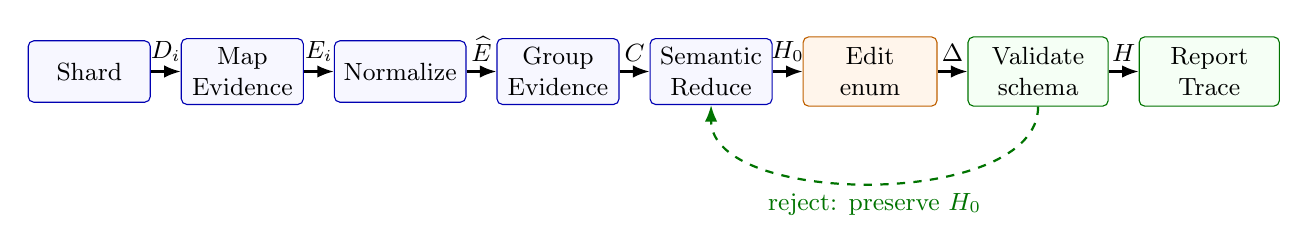
\begin{tikzpicture}[
  font=\small,
  op/.style={draw=blue!70!black, rounded corners=2pt, minimum height=0.78cm, minimum width=1.55cm, align=center, fill=blue!3},
  sys/.style={draw=green!45!black, rounded corners=2pt, minimum height=0.88cm, minimum width=1.78cm, align=center, fill=green!4},
  llm/.style={draw=orange!75!black, rounded corners=2pt, minimum height=0.88cm, minimum width=1.70cm, align=center, fill=orange!8},
  arr/.style={-{Latex[length=2.1mm]}, thick},
  note/.style={font=\small, align=center}
]
\node[op] (shard) {Shard};
\node[op, right=0.38cm of shard] (map) {Map\\Evidence};
\node[op, right=0.38cm of map] (norm) {Normalize};
\node[op, right=0.38cm of norm] (group) {Group\\Evidence};
\node[op, right=0.38cm of group] (reduce) {Semantic\\Reduce};
\node[llm, right=0.38cm of reduce] (edit) {Edit\\enum};
\node[sys, right=0.38cm of edit] (validate) {Validate\\schema};
\node[sys, right=0.38cm of validate] (report) {Report\\Trace};
\draw[arr] (shard) -- node[above,note] {$D_i$} (map);
\draw[arr] (map) -- node[above,note] {$E_i$} (norm);
\draw[arr] (norm) -- node[above,note] {$\widehat{E}$} (group);
\draw[arr] (group) -- node[above,note] {$C$} (reduce);
\draw[arr] (reduce) -- node[above,note] {$H_0$} (edit);
\draw[arr] (edit) -- node[above,note] {$\Delta$} (validate);
\draw[arr] (validate) -- node[above,note] {$H$} (report);
\draw[arr, dashed, green!45!black] (validate.south) to[out=-90,in=-90,looseness=0.8] node[below,note] {reject: preserve $H_0$} (reduce.south);
\end{tikzpicture}
\caption{\systemname{} is an operator and state-transition contract. Existing data runtimes can supply the scale-facing operators. A model may influence only the bounded \textsf{Edit} transition; system-owned \textsf{Validate} binds evidence, checks schema and consistency invariants, and preserves a valid pre-edit state on rejection. \textsf{ReportTrace} makes the committed execution auditable.}
\label{fig:operator-algebra}
\end{figure*}

The prototype maps this algebra onto a workflow/stream runtime without modifying the storage or serving engines. Dataflow stages implement the scale-facing operators; reducer plug-ins share the same candidate, hypothesis, and trace types; an OpenAI-compatible endpoint can supply \textsf{Edit} decisions; and the runtime owns evidence identifiers, edit assembly, validation, fallback, latency/token accounting, and trace capture. Thus model output cannot directly become report state. It is an untrusted proposal interpreted through the same commit/reject interface as deterministic and hybrid policies.

We evaluate the abstraction in four evidence tiers. A nine-family, ten-seed controlled matrix varies coverage, fragmentation, shared causes, concurrency, false correlation, partial evidence, overmerge, and edit admissibility under one schema and scorer. A public AIOps Challenge 2020 replay tests the evidence boundary; an AIOpsArena replay tests label-conditioned incident grouping. A 27-run runtime matrix injects invalid edits and checkpoint recovery across every controlled family; all runs reject invalid state, preserve the baseline, restore the committed digest, and replay deterministically. Finally, a single-accelerator real-online matrix repeats the same nine families and three seeds five times: at an eight-candidate budget, bounded action validation improves mean F1 from 0.7801 for the hybrid baseline to 0.8645. Within-case F1 standard deviation is zero; four proposed actions are rejected, while schema failure and fallback remain zero. A three-sample 14B checkpoint retains the gain at 0.8392 F1. These online results are mechanism evidence at two scales in one model family and endpoint stack, not cross-family or production robustness.

This paper makes three contributions:

\begin{enumerate}[leftmargin=1.6em]
\item \textbf{Operator contract.} We define a typed algebra for evidence-linked semantic reduction and specify bounded edit, validation, provenance, and recovery invariants that separate model policy from runtime state integrity.
\item \textbf{Runtime integration.} We instantiate the algebra in a workflow/stream runtime that keeps edit assembly, validation, fallback, state digests, checkpoint recovery, accounting, and replayable traces system-owned.
\item \textbf{Workloads and evidence.} We organize nine reproducible contract-obligation families, add public evidence-boundary and incident-grouping replays plus a recovery fault matrix, and report these separately from the real-online mechanism study.
\end{enumerate}

Sections~2--5 motivate and define the contract and its runtime integration; Sections~6--7 describe the workload and evaluation; Section~8 discusses implications and limitations; Section~9 covers related work.

\section{Motivation}

Operational analysis often starts with numerical aggregates but ends with semantic judgment. In an accelerator-backed LLM serving platform, a dashboard may show that p95 latency increased in one region, decode utilization saturated, scheduler queue depth grew, and errors rose for some tenants. Each observation is measurable with conventional analytics; the harder question is whether these observations are one incident, several unrelated incidents, or noise. Conventional engines provide the substrate for scans, windows, joins, and stateful aggregation, but they do not normally expose first-class incident hypotheses, evidence objects, conflict handling, or explanation traces.

LLM-enabled data tools often expose a chat interface over a database, log store, vector index, or dashboard. This is useful for ad hoc exploration, but it hides important systems structure: which context was inspected, how evidence was compressed, when follow-up queries were issued, and why a final answer should be trusted. Large-scale analysis needs explicit partitioning, bounded local evidence, semantic reduction, and traceable reports.

The missing component is a reducer-state boundary, not a new storage, dataflow, or serving engine. Spark, Flink, Ray, SQL engines, vector stores, and serving engines can retain partitioning, scheduling, indexing, and inference. The runtime hosting semantic reduction must additionally specify the evidence admitted to a reducer, the finite state effects a policy may request, the checks preceding commit, and the state and trace retained after rejection or recovery.

\section{Problem Statement}

Let partitioned observations $D$ produce a valid baseline hypothesis state $H_0$. A semantic policy may propose an edit $\Delta$, but only the runtime may publish a successor state $H$. The contract must satisfy three obligations. \emph{Eligibility}: every reducer candidate and output hypothesis is derived from typed, provenance-bearing evidence selected before model invocation. \emph{Transition integrity}: the policy has a finite action space, and schema, evidence, and cross-field invariants are checked before commit; otherwise the visible state remains $H_0$. \emph{Recovery and audit}: committed state, validator outcome, cost, and replay metadata survive checkpoint recovery and suffice to reproduce the same semantic-state digest. Scale-facing operators may compress observations before this boundary, but compression failure must be reported as missing evidence rather than hidden as reducer error.

This formulation excludes two tempting shortcuts. Generating valid JSON does not establish evidence eligibility, legal state effects, or rollback. Persisting an agent/workflow graph records control flow but does not by itself define which semantic transition is admissible. The research question is therefore not how to prompt a model to summarize data, but how a runtime admits an untrusted semantic decision into durable analysis state.

\section{\systemname{} Operator Model}

The central claim of \systemname{} is that LLM-native analysis needs standard operators, analogous in spirit to \texttt{map} and \texttt{reduce}, but with contracts for evidence, bounded semantic edits, validation, and explanation. The abstraction is not an agent prompt wrapped around a database. It is an operator model in which observations become evidence, evidence becomes reducer candidates, reducer candidates become hypotheses, and every semantic edit is either validated or rejected before it affects the report.

Let $D$ denote a collection of observations, $\mathcal{E}$ evidence objects, $\mathcal{C}$ reducer candidates, $\mathcal{H}$ hypotheses, $\Delta$ reducer edits, $\mathcal{T}$ workflow trace records, and $\mathcal{Y}$ the final report. \systemname{} composes the following operators:

\begin{align}
\mathcal{A} &= \{\textsc{Keep},\textsc{Merge},\textsc{Split},\textsc{Abstain}\} \\
\mathcal{S} &= \textsf{Shard}(D;\pi) \\
\mathcal{E} &= \bigcup_{s \in \mathcal{S}} \textsf{MapEvidence}(s;\phi) \\
\widehat{\mathcal{E}} &= \textsf{Normalize}(\mathcal{E};\sigma) \\
\mathcal{C} &= \textsf{GroupEvidence}(\widehat{\mathcal{E}};\gamma) \\
(\mathcal{H}_0,\mathcal{T}_R) &= \textsf{SemanticReduce}(\mathcal{C};\rho) \\
\Delta &= \textsf{Edit}(\mathcal{C}, \mathcal{H}_0; a), \quad a \in \mathcal{A} \\
(\mathcal{H},\mathcal{T}_V) &= \textsf{Validate}(\mathcal{H}_0,\Delta,\widehat{\mathcal{E}};V) \\
(\mathcal{Y},\mathcal{T}) &= \textsf{ReportTrace}(\mathcal{H},\widehat{\mathcal{E}},\mathcal{T}_R \cup \mathcal{T}_V;\tau).
\end{align}

The policies $\pi,\phi,\sigma,\gamma,\rho,V,\tau$ may be implemented by rules, queries, stream processors, graph algorithms, LLM calls, or hybrids. The important invariant is that only structured objects cross operator boundaries. Local findings are evidence objects rather than prompt text; reducer inputs are candidate groups rather than raw telemetry; model-backed edits are bounded actions rather than complete incident reports; and reports preserve evidence links rather than only natural-language conclusions.

This model separates the part a model may do from the part the system must own. \textsf{SemanticReduce} can be deterministic, graph-based, LLM-backed, or hybrid. When a model is used, the safer interface is often \textsf{Edit}: the model makes a bounded semantic decision such as whether two candidates should be merged, split, kept separate, or abstained from. The system then assembles the edit payload, binds evidence identifiers, checks the incident schema, verifies root and affected-service consistency, and falls back when validation fails. This is why the evaluated one-token reducer is not merely a prompt variant: it changes the reducer contract from ``generate JSON hypotheses'' to ``choose a bounded action that the system can validate.''

External data engines may implement the scale-facing operators, while LLM frameworks may implement semantic decisions or reporting. The semantic runtime composes them under one auditable evidence contract and owns the boundaries where data-plane outputs become semantic-control-plane decisions. The operators expose five contract surfaces: data engines provide shards, windows, summaries, or chunks; local findings become bounded evidence objects rather than prompt text; reducers may change strategy while preserving the incident schema and scorer; model-backed edits must pass evidence and schema validation; and \textsf{ReportTrace} ties every hypothesis to operator decisions, supporting evidence, and replay metadata.

\textbf{Shard and map evidence.} Each shard is processed locally. \textsf{MapEvidence} may compute statistics, identify anomalies, summarize logs, classify symptoms, or invoke an LLM over a bounded context. Its output is not arbitrary prose. It is an evidence object with fields such as service, tenant, region, metric, time window, observed value, baseline, severity, confidence, and source references.

\textbf{Normalize, group, and semantic reduce.} \textsf{Normalize} and \textsf{GroupEvidence} prepare evidence for global reasoning. \textsf{SemanticReduce} then merges evidence objects into higher-level hypotheses. This stage deduplicates adjacent windows, combines weak but consistent signals, separates unrelated incidents, handles contradictory evidence, and assigns confidence. The reducer may be deterministic, LLM-backed, or hybrid. Deterministic reducers are useful baselines because they are reproducible and cheap; LLM reducers are attractive when the merge requires domain language, causal reasoning, or flexible explanation.

\textbf{Edit and validate.} A model-backed reducer need not emit final hypotheses. It can instead implement \textsf{Edit}: a bounded decision over reducer candidates. In the evaluated action reducer, the model chooses only \textsc{Keep}, \textsc{Merge}, \textsc{Split}, or \textsc{Abstain}. \textsf{Validate} then checks that any proposed edit preserves evidence references, schema constraints, root and affected-service consistency, and the no-regression fallback policy. Invalid model text becomes \textsc{Abstain}; invalid edits are rejected; unsafe reducer outputs fall back to the deterministic or hybrid baseline.

\textbf{Report and trace.} \textsf{ReportTrace} turns hypotheses into operator-facing reports. The report should include the claim, supporting evidence, possible conflicting evidence, and suggested actions. It should also preserve the workflow trace so a user can inspect how the conclusion was formed.

\systemname{} differs from an agent loop because its units of parallelism, evidence compression, reduction, and reporting are explicit. It also differs from ordinary stream processing: stream windows can compute features and alerts, but semantic reduction turns local findings into a global explanation.

\begin{algorithm}[t]
\caption{\systemname{} Workflow}
\label{alg:semantic-mapreduce}
\small
\begin{algorithmic}[1]
\Require Observations $D$, policies $\pi,\phi,\sigma,\gamma,\rho,V,\tau$
\Ensure Evidence-linked incident report $\mathcal{Y}$ and workflow trace $\mathcal{T}$
\State $\mathcal{S} \gets \Call{Shard}{D;\pi}$ \Comment{partition by service, region, tenant, or time}
\State $\mathcal{E} \gets \emptyset$, $\mathcal{T} \gets \emptyset$
\ForAll{shard $s \in \mathcal{S}$}
  \State $(E_s, T_s) \gets \Call{MapEvidence}{s;\phi}$
  \State $\mathcal{E} \gets \mathcal{E} \cup E_s$
  \State $\mathcal{T} \gets \mathcal{T} \cup T_s$
\EndFor
\State $\widehat{\mathcal{E}} \gets \Call{Normalize}{\mathcal{E};\sigma}$
\State $\mathcal{C} \gets \Call{GroupEvidence}{\widehat{\mathcal{E}};\gamma}$
\State $(\mathcal{H}_0, T_R) \gets \Call{SemanticReduce}{\mathcal{C};\rho}$
\State $(\Delta, T_E) \gets \Call{Edit}{\mathcal{C},\mathcal{H}_0}$ \Comment{optional bounded edit}
\State $(\mathcal{H}, T_V) \gets \Call{Validate}{\mathcal{H}_0,\Delta,\widehat{\mathcal{E}};V}$
\State $\mathcal{T} \gets \mathcal{T} \cup T_R$
\State $\mathcal{T} \gets \mathcal{T} \cup T_E \cup T_V$
\State $\mathcal{Y} \gets \Call{ReportTrace}{\mathcal{H}, \widehat{\mathcal{E}}, \mathcal{T};\tau}$
\State \Return $(\mathcal{Y}, \mathcal{T})$
\end{algorithmic}
\end{algorithm}

Algorithm~\ref{alg:semantic-mapreduce} makes the operator vocabulary operational. The important constraint is that \textsf{SemanticReduce} consumes compact, normalized, grouped evidence objects rather than raw telemetry, and that model-backed \textsf{Edit} decisions are validated before they affect $\mathcal{H}$. This lets the runtime place expensive or policy-sensitive LLM calls at semantic boundaries instead of at every scan or filter operation.

\section{Runtime Contract and Integration}

The prototype keeps the execution boundary deliberately narrow. Storage, joins, stream windows, distributed scheduling, and model serving remain delegated to existing engines; the semantic runtime owns operator composition, evidence schemas, reducer selection, validation, and trace capture. This is the difference from simple stitching. A script can query a data engine and then call a model, but it does not define which evidence objects cross the boundary, how duplicate local alerts become one hypothesis, or how a report links back to reducer decisions.

The workflow graph is one host representation of this contract. It composes familiar stream/dataflow operators--map, filter, flatmap, key grouping, and connection--but assigns them semantic roles. Sharded maps implement \textsf{MapEvidence}; keyed stages implement \textsf{GroupEvidence}; downstream stages invoke \textsf{SemanticReduce}, optional \textsf{Edit}, \textsf{Validate}, and \textsf{ReportTrace}. Upstream systems may supply partitions, windows, feature tables, retrieved documents, or trace chunks. Downstream tools consume structured incidents and evidence-linked reports. The contract can therefore be embedded above Spark, Flink, Ray, databases, vector stores, and serving endpoints rather than replacing them.

Evidence objects are the bridge between data systems and LLM reasoning. They include shard and time-window identifiers, service/region/metric fields, local baseline statistics, anomaly type, severity, confidence, and source references. Reducers consume grouped evidence and emit the same incident schema plus a reducer trace. The evaluated implementation includes map-only and window baselines, deterministic and hybrid semantic reducers, free-form LLM reducers, and action-constrained reducers under one scorer. Changing the reducer therefore does not require rewriting the generator, mapper, report schema, or benchmark matrix. The trace records reducer metadata, detected incidents, matched and missed incident IDs, evidence summaries, failure classes, run manifests, and token estimates, so false positives and false negatives can be attributed to evidence extraction, grouping, editing, validation, or thresholding rather than to an opaque final answer.

\begin{figure*}[t]
\centering
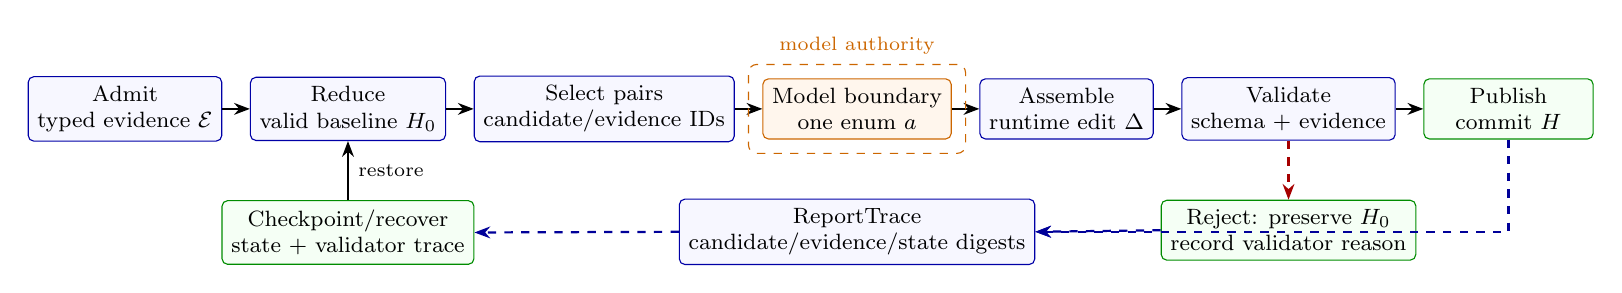
\begin{tikzpicture}[
  font=\footnotesize,
  runtime/.style={draw=blue!65!black, rounded corners=2pt, align=center, fill=blue!3, minimum height=0.72cm},
  model/.style={draw=orange!80!black, rounded corners=2pt, align=center, fill=orange!7, minimum height=0.72cm},
  state/.style={draw=green!55!black, rounded corners=2pt, align=center, fill=green!4, minimum height=0.72cm},
  arr/.style={-{Stealth[length=2mm]}, thick},
  reject/.style={-{Stealth[length=2mm]}, dashed, thick, red!65!black},
  trace/.style={-{Stealth[length=2mm]}, dashed, thick, blue!60!black}
]
\node[runtime, minimum width=2.15cm] (admit) {Admit\\typed evidence $\mathcal{E}$};
\node[runtime, minimum width=2.15cm, right=0.35cm of admit] (baseline) {Reduce\\valid baseline $H_0$};
\node[runtime, minimum width=2.2cm, right=0.35cm of baseline] (pairs) {Select pairs\\candidate/evidence IDs};
\node[model, minimum width=2.05cm, right=0.35cm of pairs] (model) {Model boundary\\one enum $a$};
\node[runtime, minimum width=2.05cm, right=0.35cm of model] (assemble) {Assemble\\runtime edit $\Delta$};
\node[runtime, minimum width=2.05cm, right=0.35cm of assemble] (validate) {Validate\\schema + evidence};
\node[state, minimum width=2.15cm, right=0.35cm of validate] (publish) {Publish\\commit $H$};

\draw[arr] (admit) -- (baseline);
\draw[arr] (baseline) -- (pairs);
\draw[arr] (pairs) -- (model);
\draw[arr] (model) -- (assemble);
\draw[arr] (assemble) -- (validate);
\draw[arr] (validate) -- (publish);

\node[state, minimum width=3.0cm, below=0.75cm of validate] (preserve) {Reject: preserve $H_0$\\record validator reason};
\node[state, minimum width=2.7cm, below=0.75cm of baseline] (checkpoint) {Checkpoint/recover\\state + validator trace};
\node[runtime, minimum width=3.3cm, below=0.75cm of model] (report) {ReportTrace\\candidate/evidence/state digests};

\draw[reject] (validate.south) -- (preserve.north);
\draw[trace] (publish.south) |- (report.east);
\draw[trace] (preserve.west) -- (report.east);
\draw[trace] (report.west) -- (checkpoint.east);
\draw[arr] (checkpoint.north) -- node[right, font=\scriptsize] {restore} (baseline.south);

\node[draw=orange!80!black, dashed, rounded corners=3pt, fit=(model), inner sep=5pt,
      label={[font=\scriptsize, orange!80!black]above:model authority}] {};
\end{tikzpicture}
\caption{Concrete reducer invocation and recovery path. Only candidate descriptions and registered evidence IDs cross the model boundary, and the model returns one action enum. The runtime constructs $\Delta$, validates it, commits $H$ or preserves $H_0$, and records digests and validator outcomes for replay. Checkpoint recovery is exercised by the model-free contract path; real-online runs retain the compatible trace fields.}
\label{fig:runtime-lifecycle}
\end{figure*}

\textbf{Invocation lifecycle.} The runtime first computes $H_0$ with the configured deterministic or hybrid reducer and selects bounded candidate pairs. Only pair descriptions and their evidence references cross the model boundary. For each pair, the endpoint returns one enum; malformed text maps to \textsc{Abstain}. The runtime converts accepted decisions into edits over a private candidate copy, rejects unknown pairs and references not drawn from both candidates, and reconstructs hypotheses from registered evidence rather than model-authored fields. \textsf{Validate} then checks candidate-evidence preservation, nonempty support, and root/affected-service consistency. A validation failure returns the configured valid baseline and records the reason. In the runtime-contract path, only validated output proceeds to the state service.

\textbf{Commit, checkpoint, and replay.} The model-free runtime-contract path wraps validated output in a checkpointable reduction service that stores hypotheses and their validator trace. Rejected edits do not invoke commit; snapshots include both state and trace; and recovery creates a new service instance before restoring the snapshot. The real-online path archives the same candidate, evidence, and committed-state digests plus whether the outcome committed or preserved the baseline. Thus the fault matrix isolates checkpoint/replay semantics without attributing them to model behavior. This is logical recovery for reducer state, not a claim of distributed exactly-once execution: upstream source replay, cross-operator transactions, and durable replicated storage remain responsibilities of the host engine.

\section{Workload and Provenance}

\subsection{Scenario}

The workload models telemetry from an NPU-backed LLM serving platform. Services include \texttt{prefill}, \texttt{decode}, \texttt{kv-cache}, \texttt{scheduler}, \texttt{router}, and \texttt{embedding}. Events include service, tenant, region, timestamp, latency, error flag, NPU utilization, queue depth, and generated metadata. The generator injects hidden incidents of three types:

\begin{itemize}[leftmargin=1.6em]
\item \textbf{Latency spike:} one service experiences elevated latency over a time window.
\item \textbf{NPU saturation:} utilization increases and may affect queueing or latency.
\item \textbf{Queue backlog:} scheduler or routing queues grow and create downstream symptoms.
\end{itemize}

The task is to recover injected incidents from event streams. A detected incident is useful only if it links to the supporting evidence and matches the hidden ground truth by type, service, region, and time.

\paragraph{Why this workload exercises the system.}

The workload is designed to stress the reducer contract rather than raw storage throughput. It has enough structure to require semantic reasoning: incidents are injected across services, regions, and time windows, while local symptoms appear as latency, error, utilization, or queue-depth changes. A single shard can observe symptoms, but the global conclusion depends on how those symptoms are merged. This matches the \systemname{} pattern.

The workload also forces the system to preserve evidence. If the reducer reports a latency spike, the report must include which shard-level candidates supported the decision. If it misses a saturation incident, the report should expose the missed incident ID. This is why the workload reports both detected and injected incidents, not only aggregate F1. The goal is not merely to score a classifier; it is to evaluate an auditable analysis workflow.

Finally, the workload is intentionally reproducible. Seeds, event counts, shard counts, top-k values, reducer names, incident reports, missed incidents, reducer traces, workflow traces, run manifests, failure classes, and token/cost accounting fields are recorded. The same matrix can be rerun when a reducer changes. This gives the prototype a benchmark harness for model-backed reducer experiments without making the current paper depend on a live model endpoint.

The semantic-merge workloads in Table~\ref{tab:workload-contract-coverage} separate positive edits from no-op and adversarial obligations. This matters because an edit protocol can appear strong if every case rewards merging. Sanity and cascade families test ordinary incident formation; concurrent and false-correlation families require separation; partial evidence distinguishes a map-coverage limit from a reducer error; and the three ambiguity families force merge, split, or abstain decisions after coverage is complete. All nine families use the same evidence schema and scorer in both the ten-seed derived matrix and the three-seed real-online matrix; the ambiguity subset is retained only as a mechanism diagnostic.

\begin{table*}[t]
\caption{Workload coverage is organized by reducer-contract obligation. All nine families have ten-seed derived matrices, three-seed runtime fault injection, and three-seed real-online action evidence.}
\label{tab:workload-contract-coverage}
\centering
\small
\begin{tabular}{@{}>{\raggedright\arraybackslash}p{0.15\textwidth}>{\raggedright\arraybackslash}p{0.22\textwidth}>{\raggedright\arraybackslash}p{0.31\textwidth}>{\raggedright\arraybackslash}p{0.23\textwidth}@{}}
\toprule
Family & Evidence condition & Required reducer behavior & Current evidence tier \\
\midrule
Single service & local, complete & preserve a trivial incident & derived + real-online \\
Cascade & cross-service, complete & fuse downstream symptoms & derived + real-online \\
Shared bottleneck & shared cause, complete & recover one common cause & derived + real-online \\
Concurrent & overlapping independent incidents & keep incident units separate & derived + real-online \\
False correlation & correlated but unrelated symptoms & reject a spurious merge & derived + real-online \\
Partial evidence & root observation absent & expose coverage/inference boundary & derived + real-online \\
Ambiguous overmerge & candidate too coarse & split or safely abstain & derived + real-online \\
Disconnected merge & one incident fragmented by grouping & accept evidence-preserving merges & derived + real-online \\
Temporal split & one incident spans candidate windows & merge without losing temporal support & derived + real-online \\
\bottomrule
\end{tabular}
\end{table*}

\subsection{Pipeline and Implementation}

The workload instantiates the operator model directly. \textsf{Shard} partitions telemetry by shard count, service, region, and time. \textsf{MapEvidence} and \textsf{Normalize} turn local anomalies into scored evidence objects, and \textsf{GroupEvidence} clusters candidates by incident type, service, region, and temporal overlap. \textsf{SemanticReduce} then emits hypotheses through map-only, window, deterministic, hybrid, stubbed, or model-backed reducers. Candidate-level and one-token action reducers exercise \textsf{Edit} and \textsf{Validate}: the model proposes bounded actions, while the system assembles evidence-linked edits, checks schema and service invariants, and falls back when required. \textsf{ReportTrace} scores hypotheses, records matched and missed incidents, classifies reducer failures, and emits per-run reports.

The workload reports precision, recall, F1, throughput, map latency, reduce latency, detected incidents, injected incidents, and missed incidents. Reports also include seed, top-k, reducer name, and incident matching metadata.

The implementation has three components. The generator creates synthetic telemetry and hidden incidents. The map stage implements \textsf{Shard}, \textsf{MapEvidence}, and \textsf{Normalize} by partitioning events, computing local summaries, and producing anomaly candidates. The reducer implements \textsf{GroupEvidence} and \textsf{SemanticReduce} over shard summaries. The default reducer is deterministic: it clusters candidates using incident type, service, region, and temporal overlap. The map-only and window-aggregation reducers are diagnostic baselines that approximate alert-only and windowed-analytics workflows without incident-level semantic reduction. The \texttt{llm-stub} reducer is an interface placeholder that exercises the same resolver and report path while delegating to the deterministic reducer.

The report schema is deliberately richer than the minimum needed for precision and recall. It includes the map policy, reducer name, seed, top-k, injected incidents, detected incidents, matched incident IDs, and missed incidents. This enables per-run diagnosis of operator behavior. When a run misses an incident, the missed incident ID is preserved in the report rather than disappearing into the aggregate recall number; when a map policy changes, the same reducer and scorer can be replayed over the new evidence stream.

The workload is designed to make reducer behavior reproducible without placing environment-management details in the paper body. Each experiment records the workload scale, shard count, seed, reducer, top-k budget, detected incidents, missed incidents, and latency measurements. This provenance is sufficient to distinguish algorithmic changes in the reducer from changes in input generation or scoring. The accompanying artifact contains the implementation and per-run records needed to rerun the study.

\section{Evaluation}

\subsection{Setup and Scope}

Representative seed-7 scale checks process 50K events/16 shards at 105.8K events/s and 100K/32 at 101.6K events/s. Both detect all four incidents. \textsf{MapEvidence} takes 72.94 and 169.61 ms, whereas deterministic reduction over compact evidence takes 0.35 and 0.31 ms. These are timing sanity checks, not the quality matrix; they show that doubling events and shards roughly doubles map time while reduction remains sub-millisecond in these runs.

The evaluation follows the operator contract rather than a single leaderboard. Q1 asks whether the workload exposes the right semantic object: incident hypotheses rather than alert fragments. Q2 asks whether \textsf{MapEvidence} surfaces enough evidence for any reducer, using coverage gates. Q3 asks whether reducer variants improve under a fixed generator, evidence schema, scorer, and report format. Q4 asks whether adjacent frameworks are substrates or whether they supply the missing semantic-reduction contract. Q5 asks whether a live model can be admitted as bounded \textsf{Edit}, rather than free-form \textsf{SemanticReduce}. This evidence ladder prevents the F1 tables from becoming a generic ML benchmark: precision, recall, and F1 check whether evidence objects are preserved, grouped, and reduced into the right incident unit. Unless explicitly labeled real-online, F1 and seed-matrix results in this section are derived artifacts from recorded workload reports; the real-online rows support live reducer-interface, validation, latency, and token-accounting claims only. The experiments are not tuned cluster deployments of Spark, Flink, Ray, LangGraph, LlamaIndex, or AutoGen.

The artifact also includes a separate shared-workload probe from a pinned workload submodule. Across seeds 7, 11, and 13, the probe generates 23 canonical LLM-serving cases per seed and 1,232 supported requests per seed, covering session-affine, RAG, long-context, tool-agent, coding-assistant, dynamic-corpus, memory-reuse, and preemption/resume surfaces. We use this probe to record workload-source provenance and to keep prototype-specific \systemname{} stress cases separate from general LLM-serving scenario catalogs. It is not used as evidence that a reducer improves incident quality.

The corresponding \systemname{} quality experiments remain repo-local because they require injected incident labels, evidence objects, reducer variants, and a common scorer. This separation prevents a common benchmark mistake: using a general workload catalog as if it were already a reducer-quality benchmark.

\subsection{Reducer Quality}

An initial 20-run sanity matrix shows why incident-level reduction is the relevant operation. Map-only reaches 0.3075 F1, window aggregation 0.7129, and the incident reducer 0.9579 while reducing average detections from 7.05 to 4.15 at 0.9750 recall. F1 is therefore a contract-level metric here: it is high only when the workflow preserves enough evidence and emits the correct incident unit with traceable matches. The nine-family suite below is the harder and submission-facing derived matrix.

\begin{table}[t]
\caption{Semantic-merge suite across nine contract-obligation families and ten seeds (90 runs per reducer). Evidence: derived artifact.}
\label{tab:semantic-merge-suite}
\centering
\small
\begin{tabular}{lcccc}
\toprule
Reducer & Precision & Recall & F1 & Detections \\
\midrule
Map-only & 0.0519 & 0.1111 & 0.0705 & 13.97 \\
Service-local & 0.0533 & 0.1111 & 0.0717 & 13.27 \\
Window-aggregate & 0.3779 & 0.7444 & 0.4916 & 8.17 \\
Semantic-graph & 0.6485 & 0.6639 & 0.6435 & 4.97 \\
Hybrid-hint & 0.7585 & 0.8556 & 0.7796 & 4.97 \\
\texttt{llm-stub} & 0.6485 & 0.6639 & 0.6435 & 4.97 \\
\bottomrule
\end{tabular}
\end{table}

Table~\ref{tab:semantic-merge-suite} adds the semantic-merge suite. A root cause in one service can produce symptoms in dependent services, so the scorer requires the hypothesis to recover the root service, region, overlapping time, and enough affected services. The nine-family aggregate is intentionally harder than the earlier seven-family diagnostic: disconnected and temporally fragmented incidents reduce the semantic-graph aggregate to 0.6435 F1, while the hint-aware reducer reaches 0.7796. The single-service sanity case still lets map-local policies succeed, so the benchmark is not constructed to make them always fail. Each family changes one semantic contract obligation while holding the generator, evidence schema, and scorer fixed. In \emph{partial-evidence}, the hint-aware reducer raises F1 from 0.5761 to 0.8878. In \emph{ambiguous-overmerge}, complete evidence can still collapse into one candidate and therefore motivates a bounded split; disconnected and temporal families require evidence-preserving merges. These are mechanism obligations, not generic model-failure labels.

\begin{table}[t]
\caption{MapEvidence policy ablation for the deterministic incident reducer. The tail-aware policy preserves high-p95 NPU saturation evidence; mean-only corresponds to the earlier mean-utilization rule. Evidence: derived artifact.}
\label{tab:map-ablation}
\centering
\small
\begin{tabular}{llcccc}
\toprule
Config & Policy & P & R & F1 & Missed \\
\midrule
50K/16/12 & Mean & 0.9200 & 0.9750 & 0.9413 & 1/10 \\
50K/16/12 & Tail & 0.9200 & 0.9750 & 0.9413 & 1/10 \\
100K/32/16 & Mean & 0.9750 & 0.9250 & 0.9464 & 3/10 \\
100K/32/16 & Tail & 0.9800 & 0.9750 & 0.9746 & 1/10 \\
\bottomrule
\end{tabular}
\end{table}

\begin{table}[t]
\caption{Coverage gate over ten seeds. A reducer-quality comparison is meaningful only when injected incidents enter the evidence objects. Baseline-aware evidence reaches full coverage for 10K and larger settings in this workload; the 2K tail-aware setting does not. Evidence: derived artifact.}
\label{tab:coverage-gate}
\centering
\small
\begin{tabular}{llccc}
\toprule
Config & Policy & Cov. mean & Cov. min & Cand. mean \\
\midrule
2K/4/8 & Tail-aware & 0.3000 & 0.0000 & 1.9 \\
2K/4/8 & Base-aware & 0.7750 & 0.5000 & 5.1 \\
10K/8/12 & Tail-aware & 0.9250 & 0.7500 & 18.2 \\
10K/8/12 & Base-aware & 1.0000 & 1.0000 & 39.5 \\
50K/16/12 & Tail-aware & 0.9750 & 0.7500 & 48.6 \\
50K/16/12 & Base-aware & 1.0000 & 1.0000 & 97.7 \\
100K/32/16 & Tail-aware & 0.9750 & 0.7500 & 47.5 \\
100K/32/16 & Base-aware & 1.0000 & 1.0000 & 112.0 \\
\bottomrule
\end{tabular}
\end{table}

Table~\ref{tab:map-ablation} is the most important diagnostic result. The larger workload exposes a failure that is not solved by changing the reducer alone: with mean-only NPU detection, three of ten 100K runs miss at least one incident. The missed cases include NPU saturation windows whose mean utilization is diluted by surrounding normal events, even though their tail utilization is high. Adding a stricter p95 NPU signal to \textsf{MapEvidence} reduces missed runs from three to one and raises 100K F1 from 0.9464 to 0.9746.

Table~\ref{tab:coverage-gate} adds a stronger guardrail: before comparing reducers, the system should measure whether the map stage surfaced the injected incidents as evidence. A later trace-guided pass exposed a second evidence failure: low-baseline services such as routers can suffer real latency spikes whose absolute p95 remains small and whose window mean rises with the incident. A baseline-aware map policy compares each service/region window against a robust shard-local latency baseline. On the same two-size, ten-seed matrix, this policy raises the deterministic incident reducer to 1.0000 mean precision, recall, and F1, while map-only remains at 0.3500 F1 and window aggregation at 0.6366 F1. This result strengthens the operator argument: once map, evidence, and reduce are separate contracts, a failure can be localized to the evidence policy rather than vaguely attributed to ``the LLM'' or ``the reducer.''

The ablation also prevents overclaiming. Tail-aware and baseline-aware evidence policies are workload policies, not universal detectors. Baseline-aware evidence increases the number of map candidates, so it must be paired with incident-level reduction; otherwise map-only precision falls sharply. A stronger system would learn or calibrate the evidence policy from real traces.

\subsection{Substrate and Overhead Checks}

Local runtime checks show that the map stage dominates because it scans and summarizes event shards, while the deterministic reduce stage runs over compact candidates. Adjacent-framework probes with Ray-local, LangGraph-local, and LlamaIndex-docstore wrappers obtain the same F1 as the native path when they are given the same evidence objects, reducer, scorer, and report format. These probes are not leaderboards over those systems. They support the narrower systems claim that existing substrates can carry the computation, but this workload still needs the evidence-linked reducer contract and audit trail.

\begin{table}[t]
\caption{Runtime-contract fault matrix: nine families $\times$ three seeds. Every row injects an invalid edit and checkpoint recovery. Evidence: derived artifact.}
\label{tab:runtime-contract}
\centering
\small
\begin{tabular}{lr}
\toprule
Invariant & Passes / runs \\
\midrule
Valid transition commits & 27 / 27 \\
Invalid edit rejected & 27 / 27 \\
Baseline state preserved & 27 / 27 \\
Checkpoint digest restored & 27 / 27 \\
Trace replay deterministic & 27 / 27 \\
\bottomrule
\end{tabular}
\end{table}

Table~\ref{tab:runtime-contract} isolates runtime behavior from model quality. For each family/seed, the harness materializes a valid baseline in a checkpointable shared-state service, validates a legal transition, injects an edit with missing candidate evidence, and invokes checkpoint recovery. The runtime records the candidate, evidence, committed-state digests, commit/reject outcome, service revision, and replay identifier. All invalid edits preserve the canonical baseline, and all recovered and replayed states match the committed digest. This is not a claim of distributed exactly-once fault tolerance: it establishes that the implemented operator boundary has an executable recovery contract rather than relying on prompt compliance.

\begin{table}[t]
\caption{External public-data checks. AIOps 2020 tests evidence coverage; AIOpsArena tests reducer grouping with label-conditioned evidence. Evidence: replay.}
\label{tab:public-replay}
\centering
\small
\begin{tabular}{lr}
\toprule
Field & Result \\
\midrule
Labeled / negative windows & 4 / 8 \\
Detected labeled windows & 2 / 4 \\
False-positive windows & 0 / 8 \\
Precision / recall / F1 & 1.000 / 0.500 / 0.667 \\
Raw rows republished & no \\
\midrule
AIOpsArena label rows / episodes & 23 / 8 \\
Map-only / window F1 & 0.516 / 0.800 \\
Service-local / semantic F1 & 1.000 / 1.000 \\
Scope & reducer-only, label-conditioned \\
\bottomrule
\end{tabular}
\end{table}

Table~\ref{tab:public-replay} replaces source availability with two scoped public-data replays. The AIOps 2020 runner reads the official daily ZIP in place, maps Docker/Oracle metrics to typed evidence using a fixed median/MAD gate, and archives only source references, evidence identifiers, scores, and provenance. Two CPU-fault windows are detected without false positives; a weak CPU shift and a window with insufficient samples are missed. We retain these misses because they expose the intended boundary: \textsf{SemanticReduce} cannot repair absent or weak \textsf{MapEvidence}.

AIOpsArena~\cite{aiopsarena2024dataset} supplies a different missing label: its complex case records 23 injected component instances that natively collapse, by timestamp, service, failure type, and duration, into eight incident episodes. We convert each public label row to an evidence unit but withhold episode identifiers from reducers. Map-only emits 23 fragments; window aggregation merges two distinct simultaneous episodes and reaches 0.800 F1; service-local and semantic reduction each recover the eight episode units. This is an oracle/label-conditioned reducer-only replay, not end-to-end anomaly detection or evidence that an LLM generalizes to production. Its value is narrower: an external dataset now exercises and scores the output unit of \textsf{SemanticReduce}, while the AIOps 2020 misses continue to bound the upstream evidence claim.

\subsection{Bounded-Edit Online Evaluation}

The real-online runs attach the same reducer contract to a live OpenAI-compatible endpoint. A smoke run served a 7B instruction-tuned model on one accelerator and completed 8/8 measured streaming requests after warmup, with mean TTFT 65.68 ms, mean TPOT 19.79 ms, and 45.71 output tokens/s. These numbers validate endpoint integration and measurement plumbing rather than SOTA serving performance. Earlier same-seed reducer probes exposed two preconditions for meaningful live LLM comparison. First, if map evidence misses incidents, no downstream reducer can recover them: a 2K/4-shard smoke produced F1 0.4000 because three injected incidents had zero overlapping map candidates. Second, asking a model to emit full reducer JSON is the wrong interface: full-evidence prompting returned legal JSON while losing incident units, and free-form candidate editors sometimes produced invalid structure or unsafe edits. The final live probe therefore focuses on the constrained \textsf{Edit}+\textsf{Validate} interface in Table~\ref{tab:pairwise-action-online}. This makes the live path an admission test for a model-backed operator: a model action is useful only if it clears coverage, schema, evidence-reference, and fallback checks under the same scorer.

\begin{table*}[t]
\caption{One-token pairwise action probe across nine families and three seeds at candidate budget 8. The primary 7B endpoint uses five samples (135 runs/reducer); the 14B checkpoint uses three (81 runs/reducer). ``Bad'' columns count invalid action/schema outputs; FB is fallback. Evidence: real-online.}
\label{tab:pairwise-action-online}
\centering
\small
\begin{tabular*}{\textwidth}{@{\extracolsep{\fill}}lrrrrrrrrrr}
\toprule
Reducer & P & R & F1 & Supp. R & ms & Tok. & Edit & Bad act. & Bad sch. & FB \\
\midrule
Hybrid hint & 0.7692 & 0.8426 & 0.7801 & 0.7810 & 0.23 & 0.0 & 0.0 & 0 & 0 & 0 \\
Validated pairwise & 0.7881 & 0.8426 & 0.7932 & 0.7948 & 1980.49 & 276.0 & 0.13 & 0 & 39 & 39 \\
Validated action (7B) & 0.8975 & 0.8426 & 0.8645 & 0.8672 & 102.73 & 260.9 & 0.81 & 4 & 0 & 0 \\
\midrule
Hybrid hint (14B) & 0.7692 & 0.8426 & 0.7801 & 0.7810 & 0.24 & 0.0 & 0.0 & 0 & 0 & 0 \\
Validated pairwise (14B) & 0.7948 & 0.8426 & 0.7977 & 0.7999 & 3056.63 & 308.9 & 0.17 & 0 & 12 & 12 \\
Validated action (14B) & 0.8549 & 0.8426 & 0.8392 & 0.8365 & 187.02 & 261.1 & 0.56 & 2 & 0 & 0 \\
\bottomrule
\end{tabular*}
\end{table*}

A follow-up pairwise edit probe narrows the interface further. Instead of asking the model to rewrite complete candidates, the reducer proposes short candidate pairs. The free-form version asks for a JSON decision list; the action version restricts each answer to \texttt{KEEP}, \texttt{MERGE}, \texttt{SPLIT}, or \texttt{ABSTAIN}, and the runtime constructs the edit payload. Table~\ref{tab:pairwise-action-online} expands the earlier hardcase probe to all nine families. On the primary endpoint, the action path raises pooled F1 from 0.7801 to 0.8645 and support recall from 0.7810 to 0.8672. Treating the 27 scenario--seed means, not the 135 repeated rows, as paired units gives a mean F1 difference of $+0.0844$ (paired-bootstrap 95\% CI: $0.0328$--$0.1449$; 10,000 draws). Within-case F1 standard deviation is zero and exact action agreement averages 0.9926. The runtime rejects four inadmissible proposed actions; no output violates schema and no run falls back. Free-form validated decisions reach only 0.7932 F1 and trigger 39 schema-preserving fallbacks.

The second checkpoint holds the workload, candidate generator, validator, scorer, and endpoint stack fixed while increasing model scale within the same family. Its action path reaches 0.8392 F1 versus 0.7801 for the hybrid baseline; the same 27-unit analysis gives $+0.0591$ (95\% CI: $0.0147$--$0.1149$). It has two rejected actions, zero schema failures, and zero fallback. The action path calls the model on 48.15\% of rows at both scales; conditional on a call, median reducer latency is 160.0 ms (7B) and 276.2 ms (14B), with 541.8 and 542.3 provider-reported tokens. Reporting conditional cost avoids diluting model cost with no-pair rows. These are two checkpoints in one model family at temperature zero, not cross-family or production robustness.

\begin{figure*}[t]
\centering
% Generated by tools/benchmark_carrier/plot_semantic_mapreduce_quality_cost.py
% Inputs are frozen comparison_summary.json and stability_summary.json files.
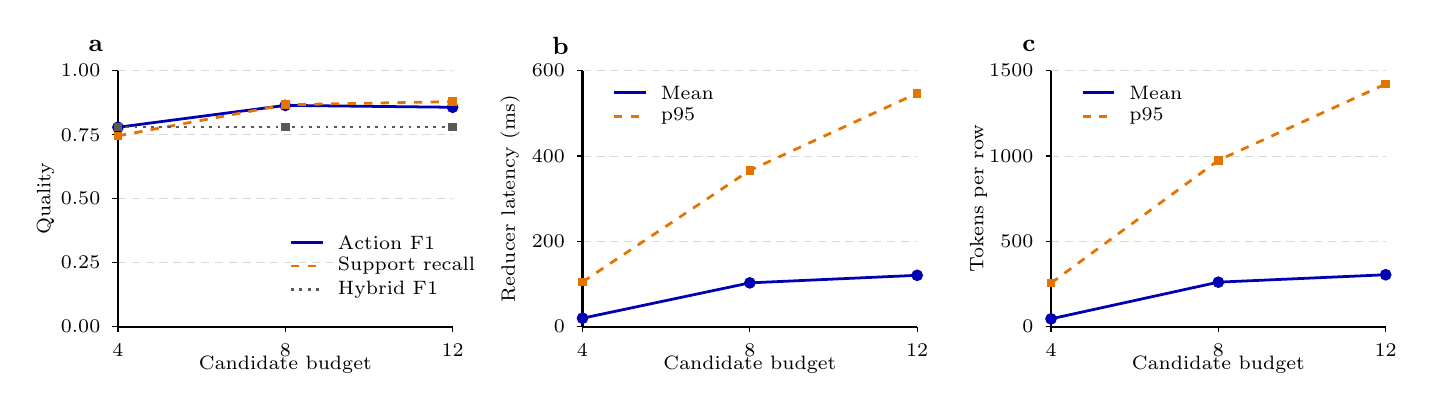
\begin{tikzpicture}[x=1cm,y=1cm]
\node[font=\bfseries\small] at (0.770,4.220) {a};
\draw[gray!30, densely dashed, line width=0.25pt] (1.050,0.650) -- (5.300,0.650);
\draw (0.980,0.650) -- (1.050,0.650);
\node[anchor=east, font=\scriptsize] at (0.950,0.650) {0.00};
\draw[gray!30, densely dashed, line width=0.25pt] (1.050,1.462) -- (5.300,1.462);
\draw (0.980,1.462) -- (1.050,1.462);
\node[anchor=east, font=\scriptsize] at (0.950,1.462) {0.25};
\draw[gray!30, densely dashed, line width=0.25pt] (1.050,2.275) -- (5.300,2.275);
\draw (0.980,2.275) -- (1.050,2.275);
\node[anchor=east, font=\scriptsize] at (0.950,2.275) {0.50};
\draw[gray!30, densely dashed, line width=0.25pt] (1.050,3.087) -- (5.300,3.087);
\draw (0.980,3.087) -- (1.050,3.087);
\node[anchor=east, font=\scriptsize] at (0.950,3.087) {0.75};
\draw[gray!30, densely dashed, line width=0.25pt] (1.050,3.900) -- (5.300,3.900);
\draw (0.980,3.900) -- (1.050,3.900);
\node[anchor=east, font=\scriptsize] at (0.950,3.900) {1.00};
\draw[thick] (1.050,0.650) -- (1.050,3.900);
\draw[thick] (1.050,0.650) -- (5.300,0.650);
\draw (1.050,0.650) -- (1.050,0.580);
\node[anchor=north, font=\scriptsize] at (1.050,0.550) {4};
\draw (3.175,0.650) -- (3.175,0.580);
\node[anchor=north, font=\scriptsize] at (3.175,0.550) {8};
\draw (5.300,0.650) -- (5.300,0.580);
\node[anchor=north, font=\scriptsize] at (5.300,0.550) {12};
\node[font=\scriptsize] at (3.175,0.170) {Candidate budget};
\node[rotate=90, font=\scriptsize] at (0.130,2.275) {Quality};
\draw[blue!70!black, solid, line width=1.0pt] (1.050,3.182) -- (3.175,3.460) -- (5.300,3.436);
\node[draw=blue!70!black, fill=blue!70!black, circle, inner sep=1.35pt] at (1.050,3.182) {};
\node[draw=blue!70!black, fill=blue!70!black, circle, inner sep=1.35pt] at (3.175,3.460) {};
\node[draw=blue!70!black, fill=blue!70!black, circle, inner sep=1.35pt] at (5.300,3.436) {};
\draw[blue!70!black, solid, line width=1.0pt] (3.250,1.720) -- (3.650,1.720);
\node[anchor=west, font=\scriptsize] at (3.720,1.720) {Action F1};
\draw[orange!90!black, dashed, line width=1.0pt] (1.050,3.073) -- (3.175,3.468) -- (5.300,3.508);
\node[draw=orange!90!black, fill=orange!90!black, rectangle, inner sep=1.35pt] at (1.050,3.073) {};
\node[draw=orange!90!black, fill=orange!90!black, rectangle, inner sep=1.35pt] at (3.175,3.468) {};
\node[draw=orange!90!black, fill=orange!90!black, rectangle, inner sep=1.35pt] at (5.300,3.508) {};
\draw[orange!90!black, dashed, line width=1.0pt] (3.250,1.420) -- (3.650,1.420);
\node[anchor=west, font=\scriptsize] at (3.720,1.420) {Support recall};
\draw[black!65, dotted, line width=1.0pt] (1.050,3.185) -- (3.175,3.185) -- (5.300,3.185);
\node[draw=black!65, fill=black!65, rectangle, inner sep=1.35pt] at (1.050,3.185) {};
\node[draw=black!65, fill=black!65, rectangle, inner sep=1.35pt] at (3.175,3.185) {};
\node[draw=black!65, fill=black!65, rectangle, inner sep=1.35pt] at (5.300,3.185) {};
\draw[black!65, dotted, line width=1.0pt] (3.250,1.120) -- (3.650,1.120);
\node[anchor=west, font=\scriptsize] at (3.720,1.120) {Hybrid F1};
\node[font=\bfseries\small] at (6.670,4.220) {b};
\draw[gray!30, densely dashed, line width=0.25pt] (6.950,0.650) -- (11.200,0.650);
\draw (6.880,0.650) -- (6.950,0.650);
\node[anchor=east, font=\scriptsize] at (6.850,0.650) {0};
\draw[gray!30, densely dashed, line width=0.25pt] (6.950,1.733) -- (11.200,1.733);
\draw (6.880,1.733) -- (6.950,1.733);
\node[anchor=east, font=\scriptsize] at (6.850,1.733) {200};
\draw[gray!30, densely dashed, line width=0.25pt] (6.950,2.817) -- (11.200,2.817);
\draw (6.880,2.817) -- (6.950,2.817);
\node[anchor=east, font=\scriptsize] at (6.850,2.817) {400};
\draw[gray!30, densely dashed, line width=0.25pt] (6.950,3.900) -- (11.200,3.900);
\draw (6.880,3.900) -- (6.950,3.900);
\node[anchor=east, font=\scriptsize] at (6.850,3.900) {600};
\draw[thick] (6.950,0.650) -- (6.950,3.900);
\draw[thick] (6.950,0.650) -- (11.200,0.650);
\draw (6.950,0.650) -- (6.950,0.580);
\node[anchor=north, font=\scriptsize] at (6.950,0.550) {4};
\draw (9.075,0.650) -- (9.075,0.580);
\node[anchor=north, font=\scriptsize] at (9.075,0.550) {8};
\draw (11.200,0.650) -- (11.200,0.580);
\node[anchor=north, font=\scriptsize] at (11.200,0.550) {12};
\node[font=\scriptsize] at (9.075,0.170) {Candidate budget};
\node[rotate=90, font=\scriptsize] at (6.030,2.275) {Reducer latency (ms)};
\draw[blue!70!black, solid, line width=1.0pt] (6.950,0.757) -- (9.075,1.206) -- (11.200,1.302);
\node[draw=blue!70!black, fill=blue!70!black, circle, inner sep=1.35pt] at (6.950,0.757) {};
\node[draw=blue!70!black, fill=blue!70!black, circle, inner sep=1.35pt] at (9.075,1.206) {};
\node[draw=blue!70!black, fill=blue!70!black, circle, inner sep=1.35pt] at (11.200,1.302) {};
\draw[blue!70!black, solid, line width=1.0pt] (7.350,3.620) -- (7.750,3.620);
\node[anchor=west, font=\scriptsize] at (7.820,3.620) {Mean};
\draw[orange!90!black, dashed, line width=1.0pt] (6.950,1.218) -- (9.075,2.635) -- (11.200,3.614);
\node[draw=orange!90!black, fill=orange!90!black, rectangle, inner sep=1.35pt] at (6.950,1.218) {};
\node[draw=orange!90!black, fill=orange!90!black, rectangle, inner sep=1.35pt] at (9.075,2.635) {};
\node[draw=orange!90!black, fill=orange!90!black, rectangle, inner sep=1.35pt] at (11.200,3.614) {};
\draw[orange!90!black, dashed, line width=1.0pt] (7.350,3.320) -- (7.750,3.320);
\node[anchor=west, font=\scriptsize] at (7.820,3.320) {p95};
\node[font=\bfseries\small] at (12.620,4.220) {c};
\draw[gray!30, densely dashed, line width=0.25pt] (12.900,0.650) -- (17.150,0.650);
\draw (12.830,0.650) -- (12.900,0.650);
\node[anchor=east, font=\scriptsize] at (12.800,0.650) {0};
\draw[gray!30, densely dashed, line width=0.25pt] (12.900,1.733) -- (17.150,1.733);
\draw (12.830,1.733) -- (12.900,1.733);
\node[anchor=east, font=\scriptsize] at (12.800,1.733) {500};
\draw[gray!30, densely dashed, line width=0.25pt] (12.900,2.817) -- (17.150,2.817);
\draw (12.830,2.817) -- (12.900,2.817);
\node[anchor=east, font=\scriptsize] at (12.800,2.817) {1000};
\draw[gray!30, densely dashed, line width=0.25pt] (12.900,3.900) -- (17.150,3.900);
\draw (12.830,3.900) -- (12.900,3.900);
\node[anchor=east, font=\scriptsize] at (12.800,3.900) {1500};
\draw[thick] (12.900,0.650) -- (12.900,3.900);
\draw[thick] (12.900,0.650) -- (17.150,0.650);
\draw (12.900,0.650) -- (12.900,0.580);
\node[anchor=north, font=\scriptsize] at (12.900,0.550) {4};
\draw (15.025,0.650) -- (15.025,0.580);
\node[anchor=north, font=\scriptsize] at (15.025,0.550) {8};
\draw (17.150,0.650) -- (17.150,0.580);
\node[anchor=north, font=\scriptsize] at (17.150,0.550) {12};
\node[font=\scriptsize] at (15.025,0.170) {Candidate budget};
\node[rotate=90, font=\scriptsize] at (11.980,2.275) {Tokens per row};
\draw[blue!70!black, solid, line width=1.0pt] (12.900,0.749) -- (15.025,1.215) -- (17.150,1.309);
\node[draw=blue!70!black, fill=blue!70!black, circle, inner sep=1.35pt] at (12.900,0.749) {};
\node[draw=blue!70!black, fill=blue!70!black, circle, inner sep=1.35pt] at (15.025,1.215) {};
\node[draw=blue!70!black, fill=blue!70!black, circle, inner sep=1.35pt] at (17.150,1.309) {};
\draw[blue!70!black, solid, line width=1.0pt] (13.300,3.620) -- (13.700,3.620);
\node[anchor=west, font=\scriptsize] at (13.770,3.620) {Mean};
\draw[orange!90!black, dashed, line width=1.0pt] (12.900,1.203) -- (15.025,2.762) -- (17.150,3.731);
\node[draw=orange!90!black, fill=orange!90!black, rectangle, inner sep=1.35pt] at (12.900,1.203) {};
\node[draw=orange!90!black, fill=orange!90!black, rectangle, inner sep=1.35pt] at (15.025,2.762) {};
\node[draw=orange!90!black, fill=orange!90!black, rectangle, inner sep=1.35pt] at (17.150,3.731) {};
\draw[orange!90!black, dashed, line width=1.0pt] (13.300,3.320) -- (13.700,3.320);
\node[anchor=west, font=\scriptsize] at (13.770,3.320) {p95};
\end{tikzpicture}

\caption{Measured action-reducer operating points over the frozen five-sample, nine-family matrix (135 rows per budget). (a) F1 and support-evidence recall; the dotted line is the 0.7801 hybrid F1. (b) all-row mean and p95 reducer latency. (c) all-row mean and p95 tokens, using provider usage when present and the recorded estimate otherwise. Four candidates truncate relations; eight maximize F1; twelve cost more without improving F1. Evidence: derived summaries of real-online rows.}
\Description{Three line charts over candidate budgets 4, 8, and 12. Quality peaks at budget 8, while reducer latency and token use continue increasing through budget 12.}
\label{fig:quality-cost}
\end{figure*}

Figure~\ref{fig:quality-cost} separates quality from cost rather than claiming a serving speedup. Four candidates truncate temporal relations and do not beat the baseline. Eight candidates give the highest F1; twelve add support recall but consume more tokens and tail latency without improving F1. The three points establish a measured operating boundary, not a general quality--cost frontier.

The benchmark records more than a summary score: configuration, reducer name, injected and detected incidents, matched and missed incident IDs, evidence support, latency, token estimates, and failure classes. In the 2K live smoke, for example, three injected incidents had zero overlapping map candidates; the low F1 therefore diagnoses a coverage failure, not a reducer-quality result.

The online artifact retains each bounded-action response and provider usage envelope, timestamps, request failures, replay IDs, and state digests. The stability and budget summaries are derived from those real-online rows and remain tied to their clean endpoint commits. The same-family second scale is part of the supported claim; a cross-family model or independent endpoint would further strengthen external validity but remains untested.

\subsection{Evaluation Takeaways}

The evaluation gives three lessons. First, the workload is not merely a classifier benchmark. Precision measures whether the reducer avoids inventing incidents from noisy evidence; recall measures whether the map and reduce stages preserve weak but real incidents; the missed-incident list shows which operator boundary failed. Second, the incident reducer improves quality mainly by changing the unit of output from windows to hypotheses. The output count drops toward the four injected incidents while recall remains high. Third, the map policy matters as much as the reducer: if a saturation event never becomes evidence, no downstream LLM can recover it without going back to raw telemetry.

These lessons define the role of an LLM reducer as a constrained semantic operator rather than a replacement for the pipeline. A model should not be rewarded for basic scanning, thresholding, or duplicate removal that deterministic operators already handle. Its useful role is to adjudicate ambiguous evidence groups, use service relationships to reject false positives, explain why symptoms belong together, and produce operator-facing reports from bounded evidence objects. The implemented online path exercises this contract and shows why validation is part of the system design: accepted model edits must preserve schema, evidence references, root/affected-service consistency, and cost visibility.

\section{Discussion and Limitations}
\label{sec:open-challenges}

\subsection{Scope and Open Challenges}

\systemname{} separates the semantic control plane from data and serving planes. Data engines retain scans, joins, windows, and distributed execution; serving engines retain inference. The semantic runtime owns evidence eligibility, reducer policy, hypothesis provenance, validation, recovery metadata, and trace replay. The evaluated mechanism needs no new kernels or scheduler semantics. The public replays reduce, but do not eliminate, the external-validity gap: AIOps 2020 tests evidence coverage, while AIOpsArena scores only eight label-conditioned incident groups. Remaining challenges are non-oracle external MapEvidence, production incident grouping, cross-family studies, and serving-level constrained decoding only when a validator needs it. Evaluation should continue to establish coverage before reducer quality and live cost.

\subsection{Trust Boundary and Auditability}

Auditability is the reason to make semantic reduction an operator contract. A hypothesis is trusted because it replays to eligible evidence, reducer candidates, accepted edits, validator outcomes, and failure classes---not because its prose is fluent. The model therefore receives a bounded \textsf{Edit} over candidates that already cite evidence. The system constructs the payload, checks schema and references, verifies root/affected-service consistency, records token and latency cost, and retains the pre-edit hypothesis on rejection. The live free-form/action contrast exercises this boundary directly: one-token output turns generation uncertainty into a checkable decision.

Three invariants make the contract portable. The \emph{provenance invariant} requires every hypothesis to cite \textsf{MapEvidence} identifiers; generated rationale alone cannot create support. The \emph{edit invariant} represents each post-grouping change as \texttt{KEEP}, \texttt{MERGE}, \texttt{SPLIT}, or \texttt{ABSTAIN} over existing candidates. The \emph{recovery invariant} leaves a valid pre-edit hypothesis after rejection and restores committed state by digest after checkpoint recovery. Table~\ref{tab:runtime-contract} executes these state obligations. They are stronger than JSON mode, which says nothing about evidence eligibility, the modified candidate, or recovery.

The common trace also makes negative results diagnostic. A recall loss can be classified as missing map coverage or ignored covered evidence; a precision loss as noisy evidence or an over-merge; zero accepted edits and fallback reveal when the model contributed nothing. Reducer policy may change from deterministic to hybrid or learned without changing the scorer or report interface. The artifact records coverage, matched/missed incidents, support, accepted edits, invalid actions/schemas, fallback, tokens, latency, and failure classes as contract fields. This is an audit surface, not a claim of a complete security model.

\section{Related Work}

\textbf{Execution substrates.} MapReduce, Spark, and Flink provide the substrate for large-scale batch and stream analytics, and Ray provides a general distributed runtime for AI applications~\cite{dean2004mapreduce,zaharia2012spark,carbone2015flink,moritz2018ray}. \systemname{} borrows the local/global decomposition but changes the reducer contract from fixed aggregation to semantic evidence fusion. These systems can execute or host parts of the pipeline; they do not by themselves define the evidence object, semantic edit, validation, and trace contract studied here.

\textbf{LLM data and workflow systems.} LOTUS and Palimpzest expose LLM calls as declarative or optimizable data-processing operators~\cite{patel2024semanticoperators,liu2024palimpzest}. LangGraph, LlamaIndex, and AutoGen provide useful abstractions for agents, retrieval, tool use, and multi-agent workflows~\cite{langchain2026langgraph,llamaindex2026,wu2023autogen}. \systemname{} is complementary: those systems can carry the graph, while this paper studies the reducer-state interface---evidence eligibility, finite edit authority, validator-owned commit/fallback, and replayable semantic state.

\textbf{Serving and observability.} vLLM shows how memory management and scheduling shape LLM serving performance~\cite{kwon2023vllm}. DeathStarBench, FIRM, the Illinois trace dataset, OpenTelemetry Demo, AIOps Challenge 2020, and LO2 provide service graphs, metrics, logs, traces, and fault labels~\cite{gan2019deathstarbench,qiu2020firm,qiu2020tracedataset,opentelemetry2026demo,netman2020aiopschallenge,bakhtin2025lo2}. Root-cause localization systems such as CloudRanger and MicroRank exploit service dependencies and trace contrasts~\cite{wang2018cloudranger,yu2021microrank}. We replay AIOps 2020 at the evidence boundary and AIOpsArena at the label-conditioned incident-unit boundary, but retain controlled workloads for model-backed merge/split mechanisms and broader obligation coverage.

\textbf{Data+AI platforms.} Databricks, Snowflake Cortex, and BigQuery ML integrate analytics engines with machine learning and LLM functionality. They are important reference points, but systematic product comparison is outside this paper. The distinction we claim is narrower: a runtime-owned reducer boundary can sit above multiple engines and make evidence eligibility, bounded edit authority, validator-owned commit/fallback, and replayable semantic state explicit.

\paragraph{Positioning summary.}

The closest intellectual ancestor is MapReduce itself: local processing followed by global reduction. The closest practical neighbors are stream processors, distributed AI runtimes, LLM workflow frameworks, RAG/data frameworks, and data+AI platforms. The claim is not greater scale, feature completeness, or generality; it is that LLM-native analysis needs standard evidence operators, semantic reduction, evidence-linked reporting, and workflow traces under one reproducible contract.

\section{Conclusion}

Large-scale LLM-augmented analysis needs more than fast scans and more than chat over data. \systemname{} extends map/reduce from fixed aggregation to evidence fusion: partition observations, compress evidence, reduce hypotheses, and preserve executable audit and recovery state. Nine controlled obligation families, public evidence-boundary and incident-grouping replays, and a 27-run recovery matrix distinguish evidence coverage, reducer policy, and runtime integrity. The live experiment shows the remaining systems requirement: model edits must be bounded, schema-validated, evidence-linked, and reversible before becoming committed state. This reframes the LLM as a constrained decision procedure inside an auditable reducer: the runtime owns evidence eligibility, candidate construction, validation, fallback, and replay, so model-backed edits change analysis state only through checkable actions.

\section*{Acknowledgments}
Generative AI tools were used to assist with drafting, editing, and code generation. The authors reviewed and validated the resulting text, code, experiments, and claims.

\bibliographystyle{ACM-Reference-Format}
\bibliography{references}

\end{document}
